\section{Реберная и вершинная двусвязность графа. Блоки графа, граф блоков – точек сочленения. Найти 
компоненты реберной и вершинной двусвязности, граф блоков – точек сочленения графа.}

Часто при решении прикладных задач теории графов важно, чтобы граф был
“как можно более связным”, то есть при удалении какого-то числа ребер или
вершин он также бы оставался связным. Поэтому кроме понятий связности
существуют также понятия двусвязности, k-связности.

\begin{definition}
    Две вершины в графе называются реберно двусвязными, если
    существует два маршрута с началом в первой вершине и концом во второй, в
    которых нет общих ребер (общие вершины могут быть).
\end{definition}

\begin{definition}
    Граф называется реберно двусвязным, если любые две
    вершины являются реберно двусвязными.
\end{definition}

\begin{theorem}
    В неориентированном графе отношение реберной двусвязности на
    множестве вершин является отношением эквивалентности.
\end{theorem}

\begin{definition}
    Компонентами реберной двусвязности называют его
    подграфы, множества вершин которых -- классы эквивалентности реберной
    двусвязности, а множества ребер -- множества ребер, соединяющих вершины
    соответствующих классов эквивалентности.
\end{definition}

У графа две компоненты связности: $V_1 = \set{1,2,3,4}$ и $V_2 = \set{5,6,7}$:
\begin{figure}[h]
    \centering
    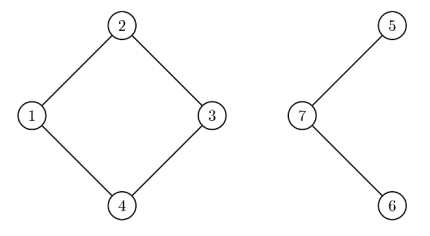
\includegraphics[scale=0.4]{14.png}
\end{figure}

Все вершины первой компоненты реберно двусвязны, поэтому эта компонента
связности является и компонентой реберной двусвязности.

Во второй компоненте никакие две вершины не являются реберно
двусвязными, поэтому каждая из них является отдельной компонентой
реберной двусвязности.

Объединение компонент реберной двусвязности не совпадает с
графом в случае, когда в графе есть мосты.

\begin{theorem}
    Компоненты реберной двусвязности графа $G(V,E)$ -- это
    компоненты связности в графе $G(V,{E}')$, где ${E}'$ получено из $E$ удалением всех
    мостов.
\end{theorem}

То есть для того, чтобы найти компоненты реберной двусвязности в графе
нужно найти все мосты, удалить их из множества ребер графа и в полученном
графе найти все компоненты связности.